\chapter{The full title of the chapter goes here}
\chaptermark{Abbreviated title for the chapter header}

\small{\textit{(Authors if you published this chapter. Cool Journal. XXX: xxx-xxx. 2014)}}

\section{Introduction}

	This is where the introduction would go. You can cite papers using the cite command, shown here \cite{Scully14}. The last bit of the document puts a references section (called references instead of ``Bibliography'').
	
	This set of files includes the bare bones for writing a thesis using latex. You need to modify the contents of each file to actually contain your thesis. For each chapter, copy this one into a new file and give it a logical name like `Chapter02.tex'.

\section{Methods}

\section{Results}

Here is an example of a table, and how to refer to it. The table in this case is table~\ref{tab:SampleTable}.

% Table 1
\begin{table}[H]
	\centering
	\caption[An example table]{This table shows an example of how you can format a table, and includes some random values for demonstration.}
	\begin{tabular}{c c c c c}
		& \multicolumn{2}{ c }{Header 1} & \multicolumn{2}{ c }{Header 2}  \\ \hline
		& CTL & Drug & CTL & Drug \\
		Variable 1 & 5 & 5 & 105 $\pm$ 5 & 101 $\pm$ 6 \\
		Variable 2 & 5 & 5 & 7.0 $\pm$ 0.6 & 8.1 $\pm$ 0.5 \\
		Variable 3 & 1000 & 1000 & 1000 & 1000 \\ \hline
	\label{tab:SampleTable}
	\end{tabular}
\end{table}

Then here is an example of a figure. The size of the figure is determined by the scale. The figure is shown in Figure~\ref{fig:SineWaves}.

% Figure 1
\begin{figure}[H]
	\centering
	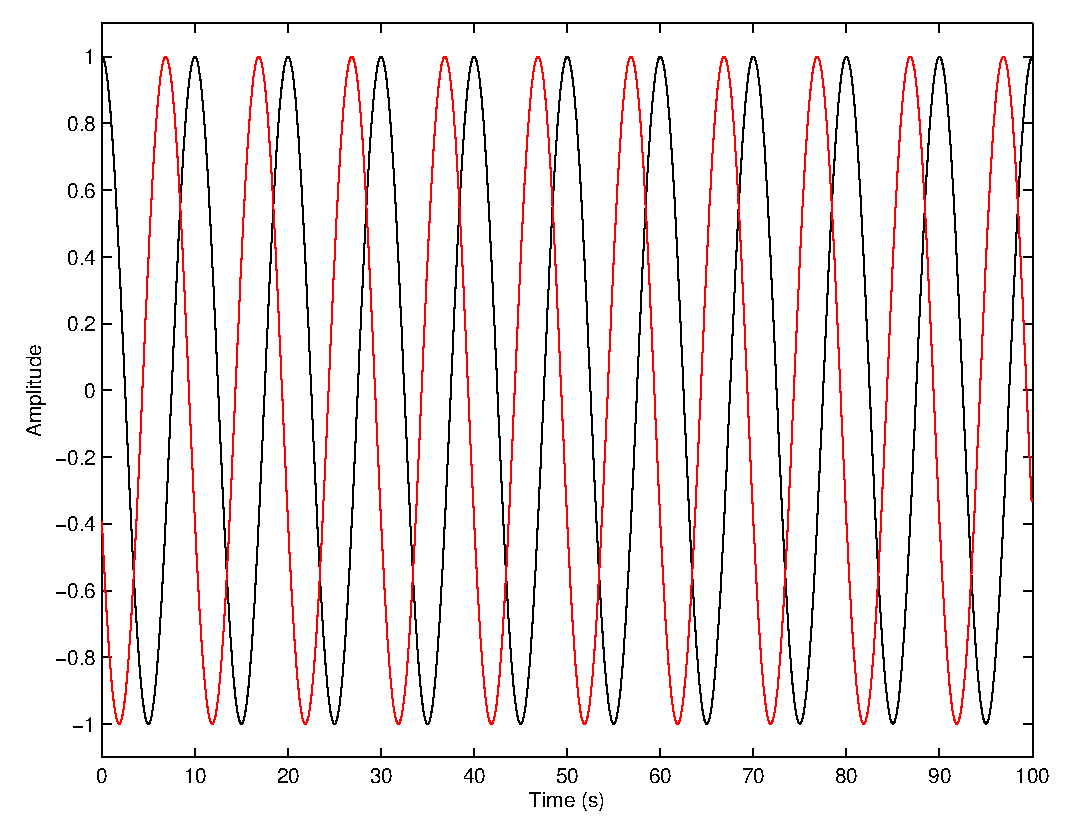
\includegraphics[scale = 0.8]{Figures/Chapter01/Figure01.eps}
	\caption[An example figure]{Two sine waves that were generated using matlab. The sine waves were generated so that their amplitude and frequency are the same, but there is a 90 degree phase shift in the \textbf{red} wave compared to the \textbf{black}.}
	\label{fig:SineWaves}
\end{figure}	

\section{Discussion}

\section{Conclusion}

\bibliographystyle{plainnat}
\renewcommand{\bibname}{References}
\bibliography{../BPK_Bibliography}